%%%%%%%%%%%%%%%%%%%%%%%%%%%%%%%%%%%%%%%%%%%%%%%%%%%%%%%%
\documentclass[12pt,a4paper]{article}% 文档格式
\usepackage{ctex,hyperref}% 输出汉字
\usepackage{times}% 英文使用Times New Roman
%%%%%%%%%%%%%%%%%%%%%%%%%%%%%%%%%%%%%%%%%%%%%%%%%%%%%%%%
\title{\fontsize{18pt}{27pt}\selectfont% 小四字号,1.5倍行距
    {\heiti% 黑体
        计算物理——Homework Week 13}}% 题目
%%%%%%%%%%%%%%%%%%%%%%%%%%%%%%%%%%%%%%%%%%%%%%%%%%%%%%%%
\author{\fontsize{12pt}{18pt}\selectfont% 小四字号,1.5倍行距
    {\fangsong% 仿宋
        白博臣、何骐多、夏营}\\% 标题栏脚注
    \fontsize{10.5pt}{15.75pt}\selectfont% 五号字号,1.5倍行距
    {\fangsong% 仿宋
        (四川大学~~~物理学拔尖计划)}}% 作者单位,“~”表示空格
%%%%%%%%%%%%%%%%%%%%%%%%%%%%%%%%%%%%%%%%%%%%%%%%%%%%%%%%
\date{}% 日期(这里避免生成日期)
%%%%%%%%%%%%%%%%%%%%%%%%%%%%%%%%%%%%%%%%%%%%%%%%%%%%%%%%
\usepackage{amsmath,amsfonts,amssymb}% 为公式输入创造条件的宏包
%%%%%%%%%%%%%%%%%%%%%%%%%%%%%%%%%%%%%%%%%%%%%%%%%%%%%%%%
\usepackage{graphicx}% 图片插入宏包
\usepackage{subfigure}% 并排子图
\usepackage{float}% 浮动环境,用于调整图片位置
\usepackage[export]{adjustbox}% 防止过宽的图片
%%%%%%%%%%%%%%%%%%%%%%%%%%%%%%%%%%%%%%%%%%%%%%%%%%%%%%%%
\usepackage{bibentry}
\usepackage{natbib}% 以上2个为参考文献宏包
%%%%%%%%%%%%%%%%%%%%%%%%%%%%%%%%%%%%%%%%%%%%%%%%%%%%%%%%
\usepackage{abstract}% 两栏文档,一栏摘要及关键字宏包
\renewcommand{\abstracttextfont}{\fangsong}% 摘要内容字体为仿宋
\renewcommand{\abstractname}{\textbf{摘\quad 要}}% 更改摘要二字的样式
%%%%%%%%%%%%%%%%%%%%%%%%%%%%%%%%%%%%%%%%%%%%%%%%%%%%%%%%
\usepackage{xcolor}% 字体颜色宏包
\newcommand{\red}[1]{\textcolor[rgb]{1.00,0.00,0.00}{#1}}
\newcommand{\blue}[1]{\textcolor[rgb]{0.00,0.00,1.00}{#1}}
\newcommand{\green}[1]{\textcolor[rgb]{0.00,1.00,0.00}{#1}}
\newcommand{\darkblue}[1]
{\textcolor[rgb]{0.00,0.00,0.50}{#1}}
\newcommand{\darkgreen}[1]
{\textcolor[rgb]{0.00,0.37,0.00}{#1}}
\newcommand{\darkred}[1]{\textcolor[rgb]{0.60,0.00,0.00}{#1}}
\newcommand{\brown}[1]{\textcolor[rgb]{0.50,0.30,0.00}{#1}}
\newcommand{\purple}[1]{\textcolor[rgb]{0.50,0.00,0.50}{#1}}% 为使用方便而编辑的新指令
%%%%%%%%%%%%%%%%%%%%%%%%%%%%%%%%%%%%%%%%%%%%%%%%%%%%%%%%
\usepackage{url}% 超链接
\usepackage{bm}% 加粗部分公式
\usepackage{multirow}
\usepackage{booktabs}
\usepackage{svg}
\usepackage{epstopdf}
\usepackage{epsfig}
\usepackage{longtable}% 长表格
\usepackage{supertabular}% 跨页表格
\usepackage{algorithm}
\usepackage{algorithmic}
\usepackage{changepage}% 换页
%%%%%%%%%%%%%%%%%%%%%%%%%%%%%%%%%%%%%%%%%%%%%%%%%%%%%%%%
\usepackage{enumerate}% 短编号
\usepackage{caption}% 设置标题
\captionsetup[figure]{name=\fontsize{10pt}{15pt}\selectfont Figure}% 设置图片编号头
\captionsetup[table]{name=\fontsize{10pt}{15pt}\selectfont Table}% 设置表格编号头
%%%%%%%%%%%%%%%%%%%%%%%%%%%%%%%%%%%%%%%%%%%%%%%%%%%%%%%%
\usepackage{indentfirst}% 中文首行缩进
\usepackage[left=2.50cm,right=2.50cm,top=2.80cm,bottom=2.50cm]{geometry}% 页边距设置
\renewcommand{\baselinestretch}{1.5}% 定义行间距(1.5)
%%%%%%%%%%%%%%%%%%%%%%%%%%%%%%%%%%%%%%%%%%%%%%%%%%%%%%%%
\usepackage{fancyhdr} %设置全文页眉、页脚的格式
\pagestyle{fancy}
\hypersetup{colorlinks=true,linkcolor=black}% 去除引用红框,改变颜色

%%%%%%%%%%%%%%%%%%%%%%%%%%%%%%%%%%%%%%%%%%%%%%%%%%%%%%%%
\newtheorem{theorem}{\indent 定理}[section]
\newtheorem{lemma}[theorem]{\indent 引理}
\newtheorem{proposition}[theorem]{\indent 命题}
\newtheorem{corollary}[theorem]{\indent 推论}
\newtheorem{definition}{\indent 定义}[section]
\newtheorem{example}{\indent 例}[section]
\newtheorem{remark}{\indent 注}[section]
\newenvironment{solution}{\begin{proof}[\indent\bf 解]}{\end{proof}}
\renewcommand{\proofname}{\indent\bf 证明}

%%%%%%%%%%%%%%%%%%%%%%%%%%%%%%%%%%%%%%%%%%%%%%%%%%%%%%%%

\begin{document}% 以下为正文内容
\maketitle% 产生标题,没有它无法显示标题
%%%%%%%%%%%%%%%%%%%%%%%%%%%%%%%%%%%%%%%%%%%%%%%%%%%%%%%%
\lhead{}% 页眉左边设为空
\chead{}% 页眉中间设为空
\rhead{}% 页眉右边设为空
\lfoot{}% 页脚左边设为空
\cfoot{\thepage}% 页脚中间显示页码
\rfoot{}% 页脚右边设为空
%%%%%%%%%%%%%%%%%%%%%%%%%%%%%%%%%%%%%%%%%%%%%%%%%%%%%%%%
\begin{figure}[h]
    \centering
    \begin{minipage}{0.32\textwidth}
        \centering
        \includegraphics[width=\linewidth]{bbc}
        \caption{白博臣}
        \label{白博臣照片}
    \end{minipage}\hfill
    \begin{minipage}{0.305\textwidth}
        \centering
        \includegraphics[width=\linewidth]{hqd}
        \caption{何骐多}
        \label{何骐多照片}
    \end{minipage}\hfill
    \begin{minipage}{0.32\textwidth}
        \centering
        \includegraphics[width=\linewidth]{xy}
        \caption{夏营}
        \label{夏营照片}
    \end{minipage}
\end{figure}


%    \begin{center}% 居中处理
%    {\textbf{Abstract}}% 英文摘要
%    \end{center}
%    \begin{adjustwidth}{1.06cm}{1.06cm}% 英文摘要内容
%        \hspace{1.5em}Attention!If you input "dif{}ferent", the computer will output "different", but if you input "dif\{\}ferent", the computer will output "dif{}ferent"
%    \end{adjustwidth}
\newpage% 从新的一页继续

\section{Problem 1}
\subsection{题目回顾}
使用传统MC方法计算积分$I=\int_{0}^{1}e^x dx$,多次重复实验,观察计算得到的积分值的分布情况,拟合并给出误差值。
\subsection{问题解答}
对于每一次积分,在被积区间的曲线上随机找1000个函数值$f(x_i)$,$0\leq j \leq n$,$0\leq x_j \leq 1$,并使用n个函数值的平均值乘上积分区间的宽度$d=1$作为单次实验的积分计算值:
\[I_j=\frac{d}{n}\cdot \sum_{j=1}^{n}f(x_j(i)) = \frac{1}{n}\cdot \sum_{j=1}^{n}e^{x_j(i)},0\leq i \leq N \]

此外,积分值$I_i$的数字特征:
\begin{align*}
    \mu_i&=E(I_i)=E(e^{x_j(i)})=\int_{0}^{1}e^x dx =e-1 = 1.718                                                         \\
    \sigma^2_i&=D(I_i)=\frac{1}{n}\cdot D(e^{x_j(i)})=\frac{1}{n}\cdot\left\{E(e^{2x_{j(i)}})-E^2(e^{x_{j(i)}})\right\} \\
    &=\frac{1}{1000}\left\{\int_{0}^{1}e^{2x}dx-\left(\int_{0}^{1}e^x dx \right)^2 \right\}=\frac{1}{1000}\left\{\frac{e^2}{2}-\frac{1}{2}-(e-1)^2\right\}
\end{align*}

误差的理论值:
\[\sigma_i=\sqrt{\frac{\frac{e^2}{2}-\frac{1}{2}-(e-1)^2}{1000}}=\frac{0.491}{1000}\]

由大数定律得,在样本足够多的情况下,积分值$I_i$的分布会趋近于正态分布:
\[I_i \~ N(\mu_i,\sigma_i^2)\~N\left(1.718,\frac{0.491^2}{1000}\right)\]

重复实验n次,可得有关单次计算值$I_i$的N元数组,可将N次实验的平均值作为最终的积分计算值:
\[I_c=\frac{1}{N}\sum_{i=1}^{N}I_i=\frac{d}{n}\cdot\frac{1}{N}\sum_{i=1}^{N}\sum_{j=1}^{n}e^{x_{j}(i)}, ~ 0\leq i \leq  N\]

也可以从实验数据的角度绘制分布曲线大致轮廓,设分布密度函数为$f(x)$,其应满足:
\[f(x)\cdot\Delta x=\frac{\Delta N}{N}\]

$\Delta x$为$x$轴上的一段固定区间,题目中所选取的$\Delta x = 0.002$,$\Delta N$是落在$\Delta x$区间上的样本点个数,$N$为总样本点个数,题目中所选取的为1000\&10000.

极限情况下的Gauss函数:

\[F(x)=\frac{1}{\sqrt{2\pi}\sigma}e^{-\frac{(x-\mu)^2}{2\sigma^2}}=\frac{1}{\sqrt{2\pi}\cdot \frac{0.491}{\sqrt{1000}}}e^{-\frac{(x-1.718)^2}{2\cdot (\frac{0.491}{\sqrt{1000}})^2}}\]

我们将实验图像与极限情况下的Gauss函数绘制在同一图像下进行对比:

\begin{figure}[htbp]
    \centering
    \includegraphics[height=8cm]{P1_1.eps}
    \caption{n=1000时,MC积分与Gauss分布}
\end{figure}

\begin{figure}[htbp]
    \centering
    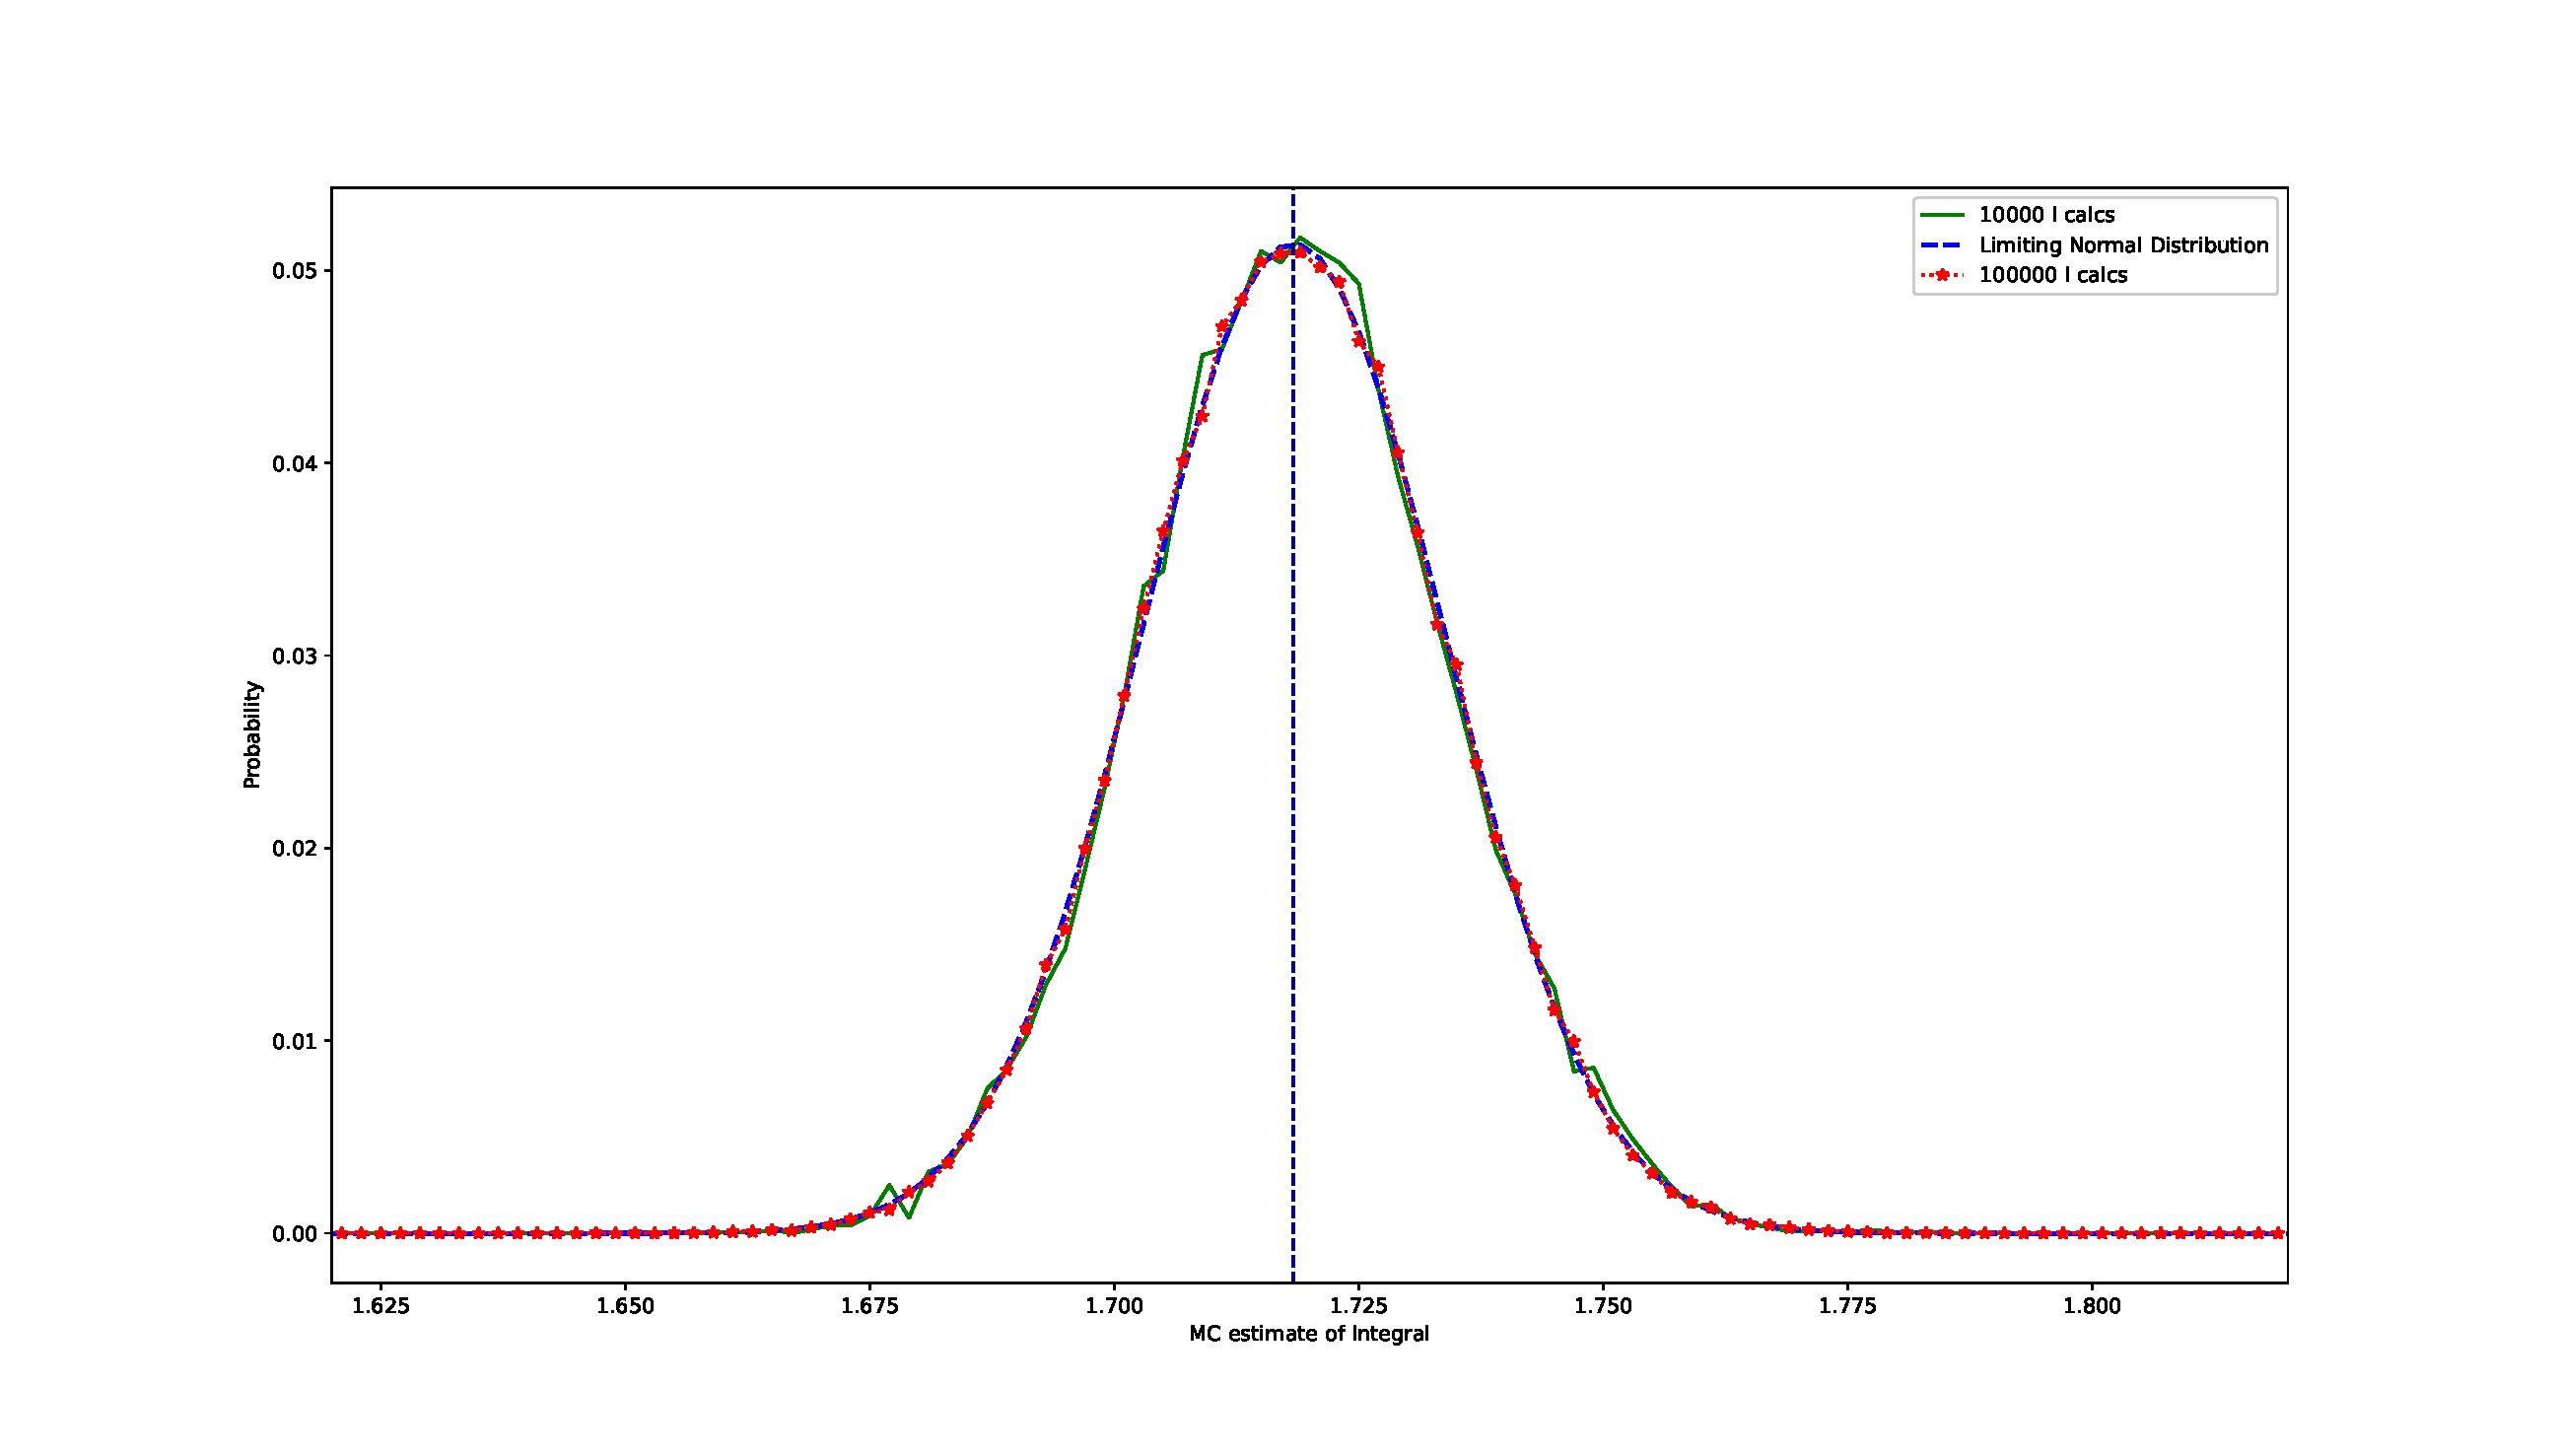
\includegraphics[height=9cm]{P1_2.eps}
    \caption{n=10000时,MC积分与Gauss分布}
\end{figure}

从上图可以看出,实验值的分布函数的极限就是Gauss函数,而且重复次数越多,实验曲线也就越贴合Gauss函数,进一步的验证了大数定律,最终积分的计算结果即为分布函数的期望:$I_c=\mu_i=1.718$

\section{Problem 2}
\subsection{题目回顾}
使用重点抽样方法来计算积分:
\[I=\int_{0}^{1}dx \frac{1}{\sqrt{x}+x}\]
\subsection{问题解答}
我们可以绘制出$\frac{1}{\sqrt{x}+x}$的图像,我们可以发现,被积函数并不平滑,在奇点0附近非常陡峭,在使用传统蒙特卡洛方法求解积分时,不利于使得更多的随机点落在区域内,从而导致计算精度下降。

一种解决方案就是做一次变量替换:
\[I=\int_{0}^{1}\frac{2\sqrt{x}}{\sqrt{x}+x}\cdot \frac{1}{2\sqrt{x}}=\int_{0}^{1}\frac{2\sqrt{x}}{\sqrt{x}+x}\cdot d\sqrt{x}=\int_{0}^{1}\frac{2x}{x^2+x}\cdot dx\]

换元处理后的被积函数明显可以观察到变得平滑了许多。

\begin{figure}[H]% 插入两张图片并且并排
    \centering
    \begin{minipage}{0.48\textwidth}
        \centering
        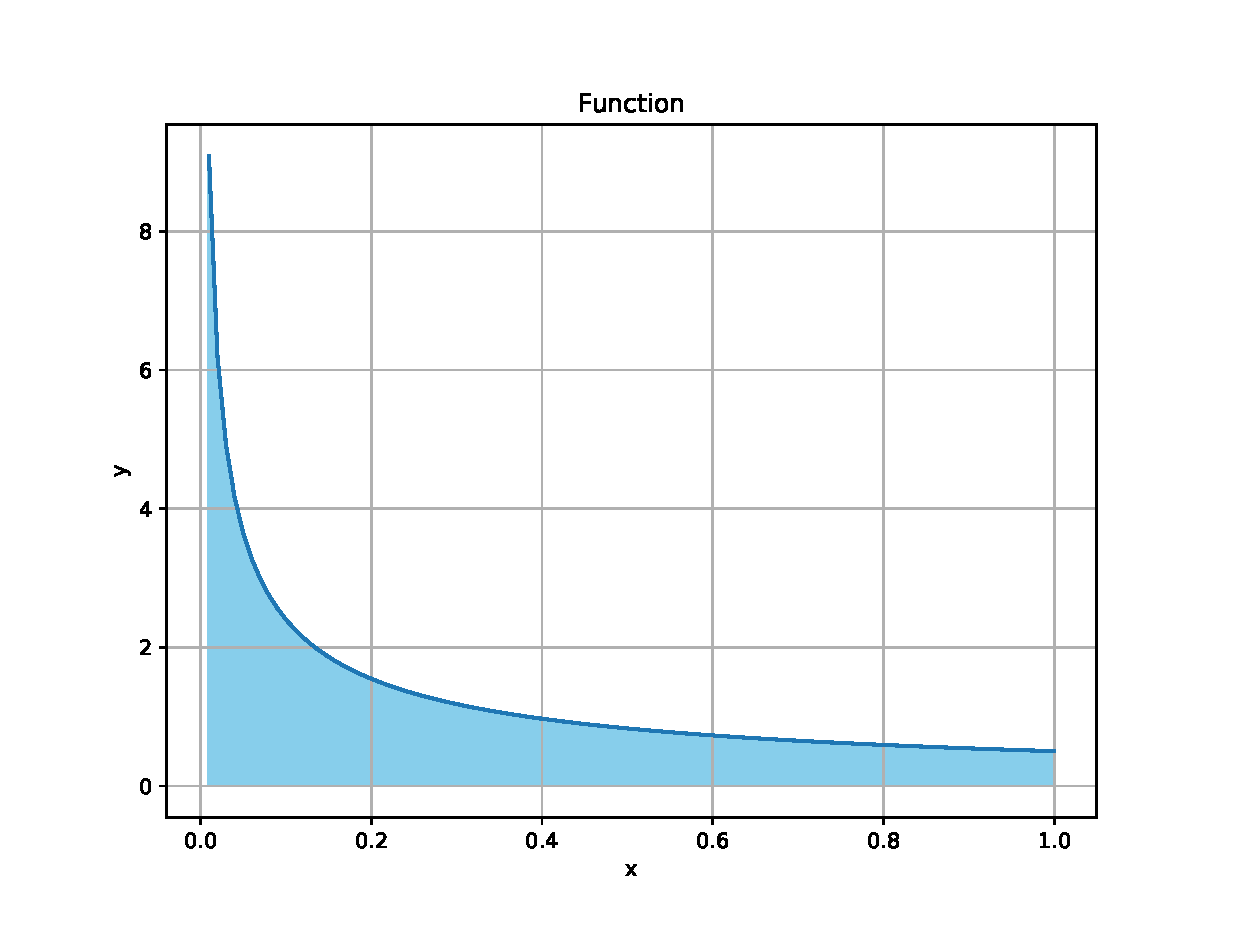
\includegraphics[width=1.1\textwidth]{function2.eps}
        \caption{\fontsize{10pt}{15pt}\selectfont $\frac{1}{\sqrt{x}+x}$函数图像}
    \end{minipage}
    \hspace{0cm}% 图片间距
    \hfill% 撑满整行
    \begin{minipage}{0.48\textwidth}
        \centering
        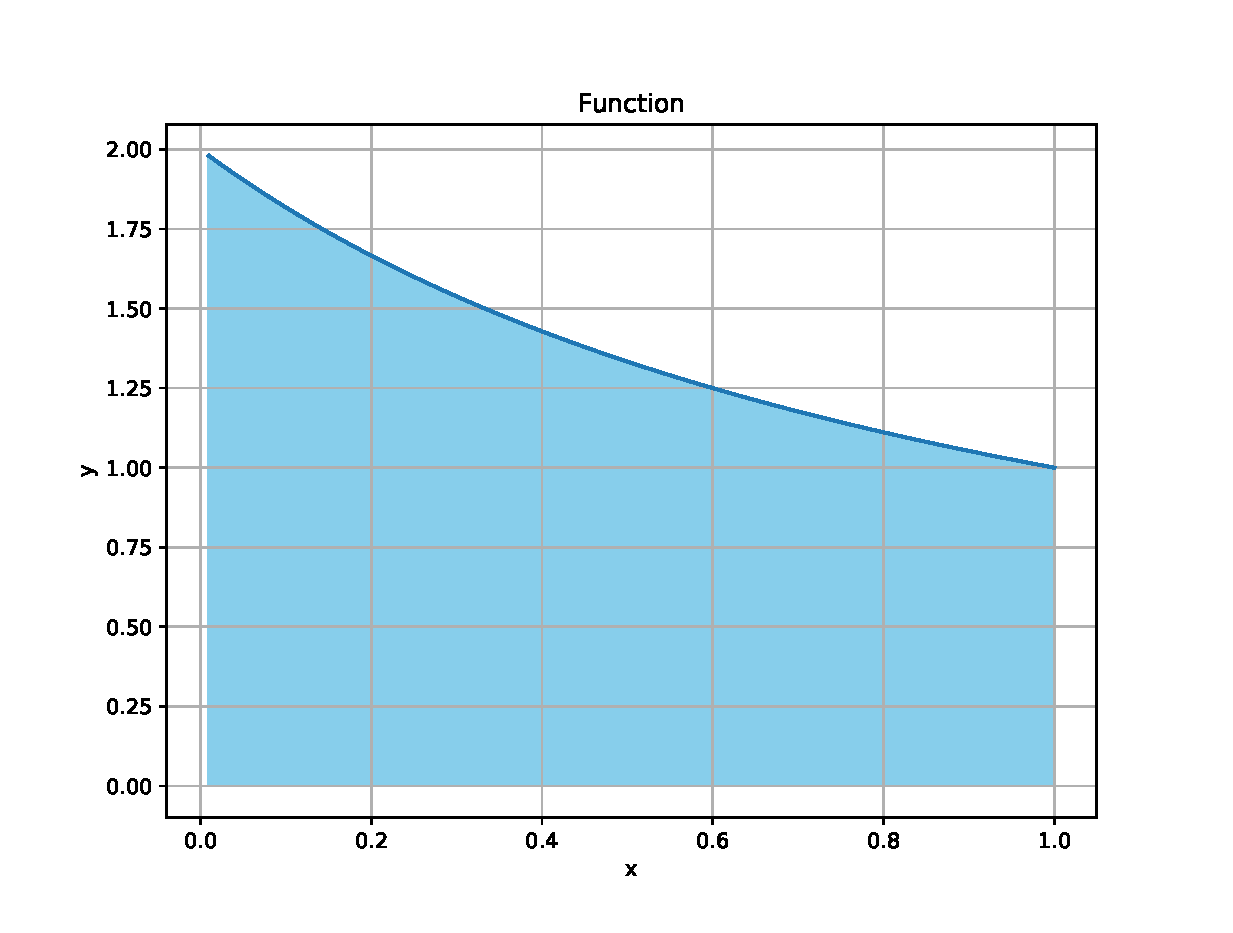
\includegraphics[width=1.1\textwidth]{function1.eps}
        \caption{\fontsize{10pt}{15pt}\selectfont $\frac{2x}{x^2+x}$函数图像}
    \end{minipage}\label{fig:figure2}
\end{figure}

在积分区间的曲线上随机找n个函数值,并使用n个函数值的平均值乘以积分区间的宽度作为单次实验的积分计算值:
\[I=\frac{d}{n}\cdot \sum_{i=1}^{n}f(x_i)=\frac{1}{n}\cdot\sum_{i=1}^{n}\frac{2x_i}{x_i^2+x_i},0\leq x_i\leq x_i\]

其积分值趋近图与误差图如下:

\begin{figure}[H]% 插入两张图片并且并排
    \centering
    \begin{minipage}{0.48\textwidth}
        \centering
        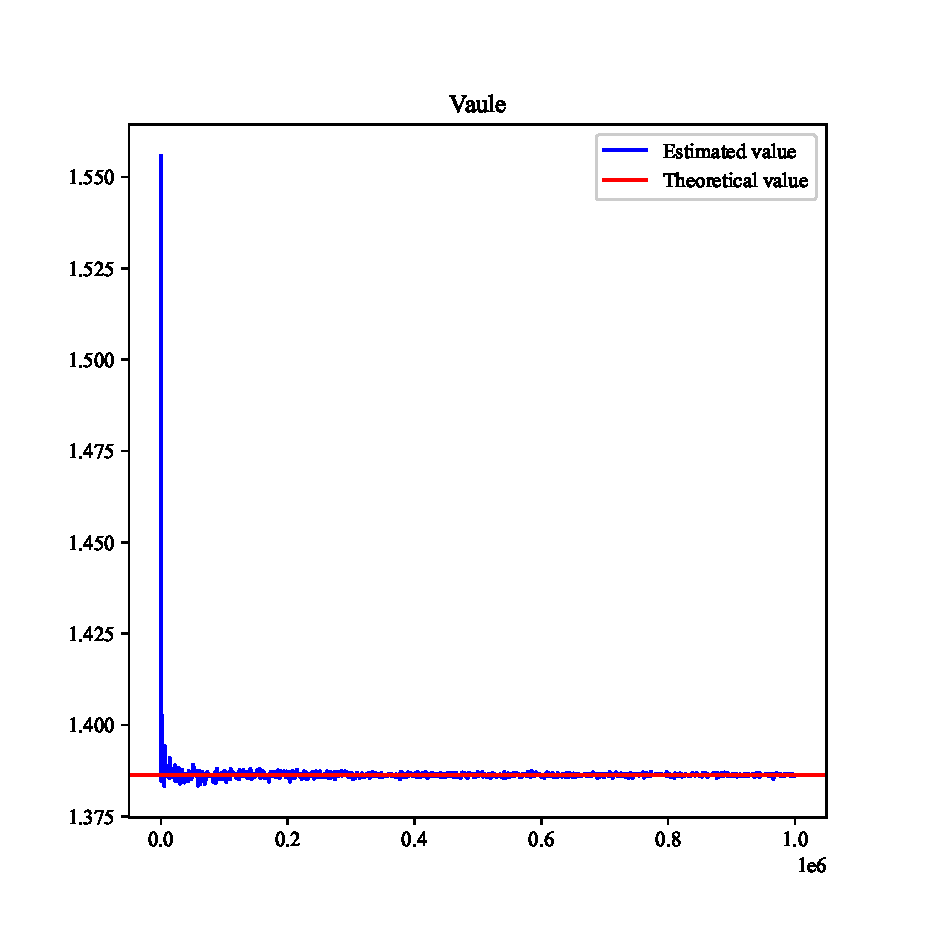
\includegraphics[width=1.1\textwidth]{函数.eps}
        \caption{\fontsize{10pt}{15pt}\selectfont MC Integration}
    \end{minipage}
    \hspace{0cm}% 图片间距
    \hfill% 撑满整行
    \begin{minipage}{0.48\textwidth}
        \centering
        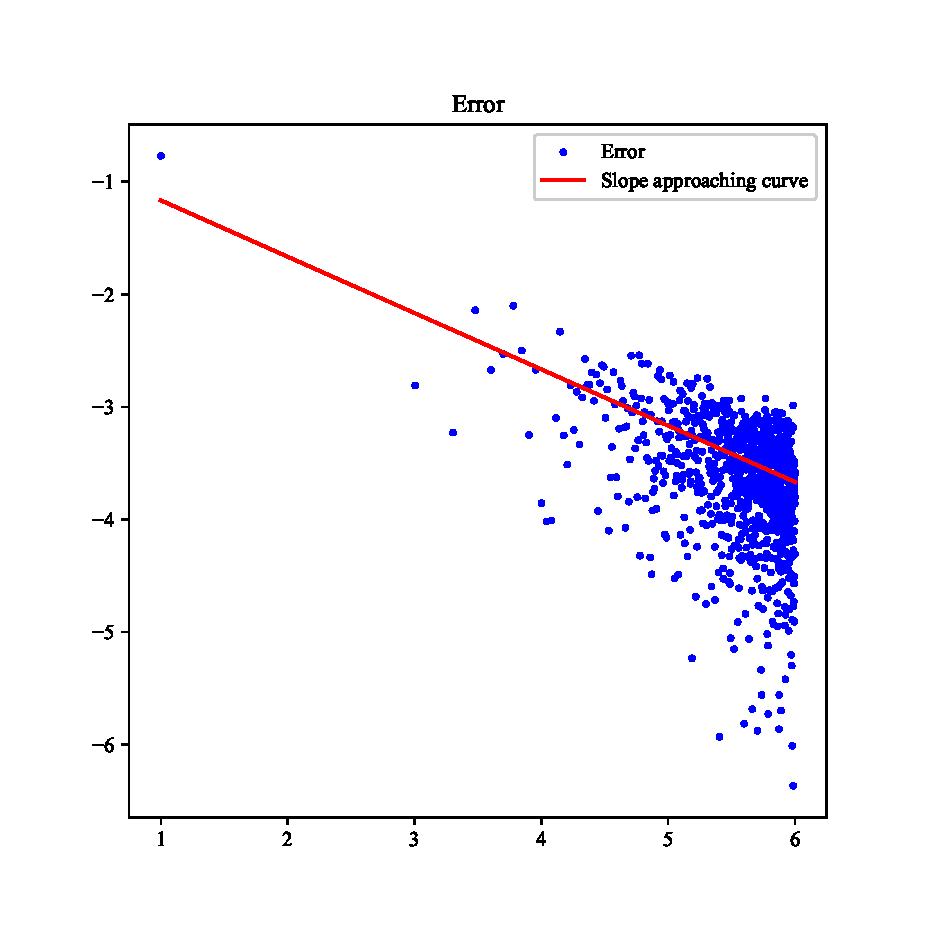
\includegraphics[width=1.1\textwidth]{误差.eps}
        \caption{\fontsize{10pt}{15pt}\selectfont 误差随随机数点数对数值变化图}
    \end{minipage}\label{fig:figure2}
\end{figure}

通过图像我们可以发现,随着样本点数的增加,我们的实验值越来越接近理论值。同时在进行换元操作后,误差衰减的速率明显加快,趋近于$N^{-\frac{1}{2}}$。

Monte Calo 方法即一个常规的二项分布,每次进行的 Bernoulli 试验为
\begin{equation*}
    x =\left\{
    \begin{aligned}
        & 0, \quad The\, point\, is\, out\, of\, the\, area\\
        & 1, \quad The\, point\, is\, in\, the\, area
    \end{aligned}
    \right.
\end{equation*}

按照棣莫佛-拉普拉斯定理,二项分布在 \(n\) 足够大时,近似为一个正态分布,有
\begin{equation*}
    P(\left| \bar{x}_\alpha - I \right| < \frac{\lambda_\alpha \sigma}{\sqrt {N}}) \approx \frac{2}{\sqrt{2 \pi}} \int^{\lambda_\alpha}_0 e^{-\frac{1}{2} t^2} dt = 1 - \alpha
\end{equation*}
其中,\(\lambda_\alpha\) 是正态分布的 \(\alpha\) 分位点,\(\sigma\) 是标准差,\(N\) 是试验次数。这表明,不等式
\begin{equation*}
    \left| \bar{x}_\alpha - I \right| < \frac{\lambda_\alpha \sigma}{\sqrt {N}}
\end{equation*}
有置信概率 \(1 - \alpha\) 成立,即 \(\bar{x}_\alpha\) 收敛到 \(I\) 的阶数为 \(O (N^{-1 / 2})\),因此,在后续的实验中应当观察到 \(\ln err - \ln N\) 图中,拟合曲线的斜率为 \(- 1 / 2\)。


\section{Problem 3}
\subsection{题目回顾}
应用分层抽样方法计算积分$I=\int_{0}^{1}dx \frac{1}{\sqrt{x}+x}$

\subsection{问题解答}
由题意得,$k=5000,n_i=10,p_i=1,\dots,5000,j=1,\dots,10$
分层抽样法将积分区域C CC分为若干个子集上的积分,使得在每个子集上的变化不大,分别计算各个子集上的积分再求和,从而提高精确度。

代入题目中的参数,得到积分估计值:
\begin{figure}[htbp]
    \centering
    \includegraphics[height=2cm]{P3.jpg}
    \caption{分层抽样积分输出结果}
\end{figure}

通过与Problem 2进行比较,我们发现分层抽样积分无论是运算速度还是精度上都要比相同样本点数量的重点抽样积分要好。

\section{Problem 4}
\subsection{问题回顾}
使用Simple MC来计算积分:
\[I=\int_{0}^{1}dx\frac{1}{\sqrt{x}+x}\]

$\left(a\right)$ 使用伪随机数来计算,理论上斜率应为$-1/2$。

$\left(b\right)$ 使用准随机书来计算,理论上斜率应为$-2/3,-1$

\subsection{问题解答}
\subsubsection{问题$\left(a\right)$解答}
对于伪随机数,有如下理论推导:

Monte Calo 方法即一个常规的二项分布,每次进行的 Bernoulli 试验为
\begin{equation*}
    x =\left\{
    \begin{aligned}
        & 0, \quad The\, point\, is\, out\, of\, the\, area\\
        & 1, \quad The\, point\, is\, in\, the\, area
    \end{aligned}
    \right.
\end{equation*}

按照棣莫佛-拉普拉斯定理,二项分布在 \(n\) 足够大时,近似为一个正态分布,有
\begin{equation*}
    P(\left| \bar{x}_\alpha - I \right| < \frac{\lambda_\alpha \sigma}{\sqrt {N}}) \approx \frac{2}{\sqrt{2 \pi}} \int^{\lambda_\alpha}_0 e^{-\frac{1}{2} t^2} dt = 1 - \alpha
\end{equation*}
其中,\(\lambda_\alpha\) 是正态分布的 \(\alpha\) 分位点,\(\sigma\) 是标准差,\(N\) 是试验次数。这表明,不等式
\begin{equation*}
    \left| \bar{x}_\alpha - I \right| < \frac{\lambda_\alpha \sigma}{\sqrt {N}}
\end{equation*}
有置信概率 \(1 - \alpha\) 成立,即 \(\bar{x}_\alpha\) 收敛到 \(I\) 的阶数为 \(O (N^{-1 / 2})\),因此,在后续的实验中应当观察到 \(\ln err - \ln N\) 图中,拟合曲线的斜率为 \(- 1 / 2\)。

使用Python编写代码后,可绘制如下图像:

\begin{figure}[htbp]
    \centering
    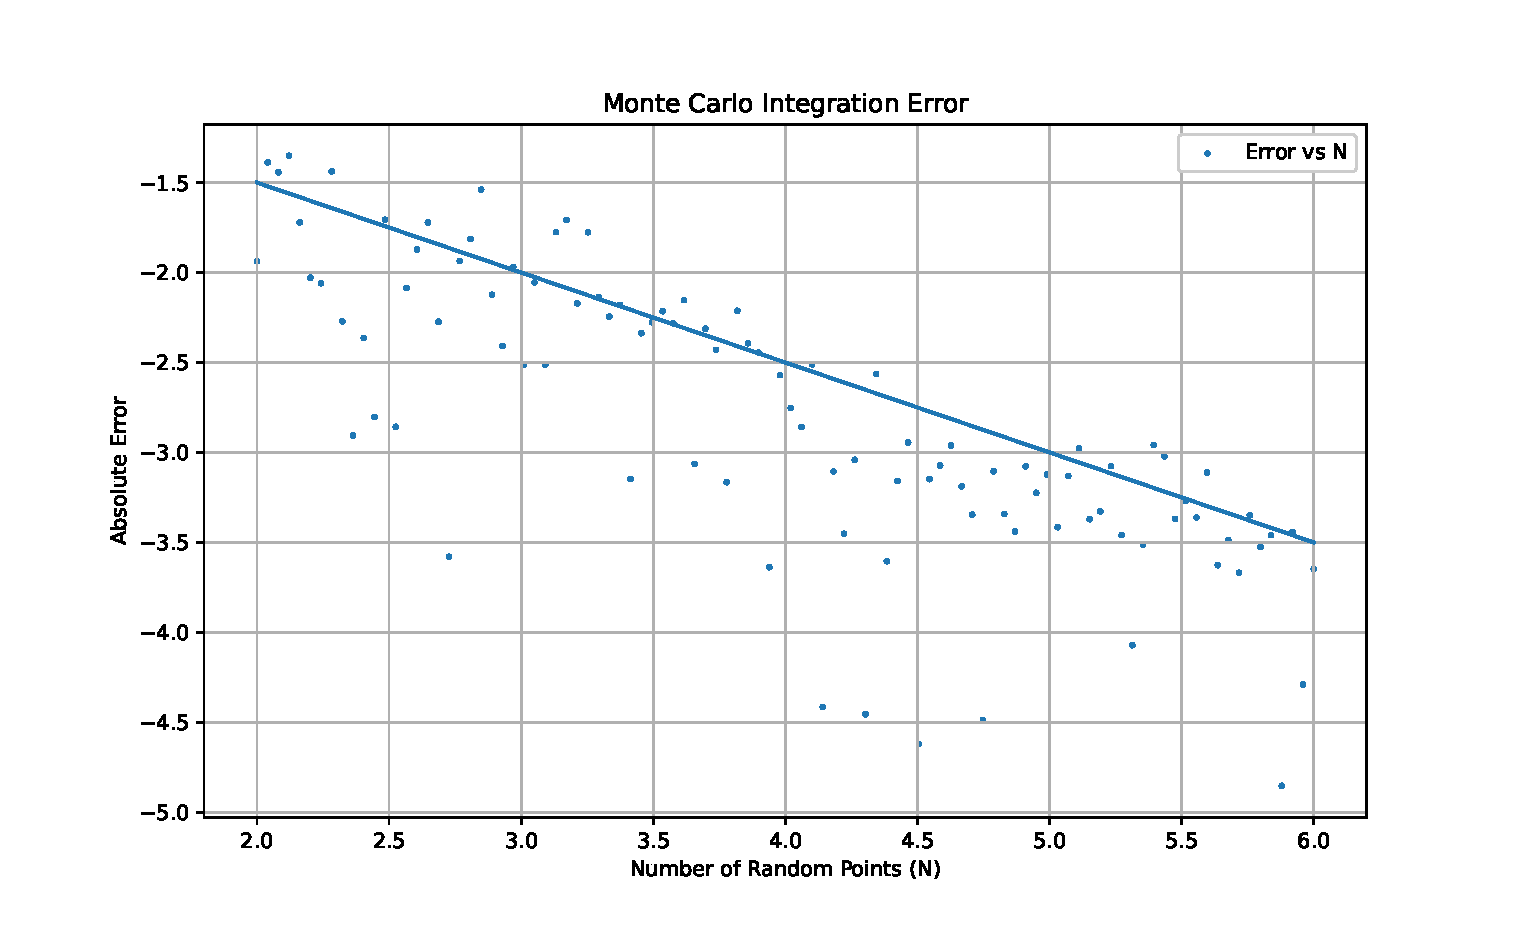
\includegraphics[height=8cm]{伪随机.eps}
    \caption{采用伪随机数(random库)计算的误差图像}
\end{figure}

可以发现斜率与$-\frac{1}{2}$契合的较好!

\subsection{问题$\left(b\right)$解答}

我们选取的Halton准随机数,代入计算后得到以下图像:

\begin{figure}[htbp]
    \centering
    \includegraphics[height=8cm]{Halton.png}
    \caption{采用准随机数(Halton)计算的误差图像}
\end{figure}

\subsection{拓展:采用真随机数(Rdrand)来进行该实验}

具体原理以及生成文档已经额外形成一个文档,这里只列出斜率曲线。

为了证明以上结果我们分别用 Random 和 RdRand 计算积分 \(\int^1_0 \frac{1}{\sqrt {x} + x} dx\) 的值,观察相对误差随点数 \(N\) 的变化。利用 \texttt{Java} 代码实现,见附件。
    
运行结果如下,

\begin{figure}[h]
    \centering
    \begin{minipage}{0.42\textwidth}
        \centering
        \includegraphics[width=\linewidth]{Random}
        \caption{Random 的运行结果}
        \label{fig:img4}
    \end{minipage}\hfill
    \begin{minipage}{0.42\textwidth}
        \centering
        \includegraphics[width=\linewidth]{RdRand}
        \caption{RdRand 的运行结果}
        \label{fig:img5}
    \end{minipage}\hfill
    \begin{minipage}{0.42\textwidth}
        \centering
        \includegraphics[width=\linewidth]{Random_k}
        \caption{Random 的斜率}
        \label{fig:img6}
    \end{minipage}\hfill
    \begin{minipage}{0.42\textwidth}
        \centering
        \includegraphics[width=\linewidth]{RdRand_k}
        \caption{RdRand 的斜率}
        \label{fig:img7}
    \end{minipage}
\end{figure}

\section{Problem 5}
\subsection{题目回顾}
使用Hit and miss Method来计算积分:
\[I=\int_{0}^{\pi}2\sin \left(2\sqrt{\pi^2-x^2}\right)\]

\subsection{问题解答}
使用Hit \& Miss Method求解积分,相当于求解被积函数在积分区间$(0,\pi)$内与x轴所围成的曲边梯形的面积。为了更好的利用随机数的周期性,样本空间的上边沿应与被积函数在区间上的最大值 $f_max=4 $相切

由样本频率趋近于概率的特性(几何概型):

\[\frac{N(hit)}{N(All Throws)}=P(Hits)=\frac{\Omega(Hit)}{\Omega(Sampling)}=\frac{\int_{0}^{\pi}2\sin \left(2\sqrt{\pi^2-x^2}\right)}{4\pi}\]

可以得到积分的计算值公式:

\[I_c=4\pi\frac{N(Hit)}{N(All Throws)}\]

使用Python编写Hit \& Miss Method程序(见Codes部分),人为设置N(All Throws)=50000,并统计N(Hit)数目,最终可以得到随机点在空间的分布如下图所示:

\begin{figure}[htbp]
    \centering
    \includegraphics[height=9cm]{P5_1.png}
    \caption{ Hit \& Miss Method可视化}
\end{figure}

\begin{figure}[htbp]
    \centering
    \includegraphics[height=9cm]{P5_2.png}
    \caption{Hit \& Miss Method积分值与准确值比较}
\end{figure}

\section{Problem 6}
\subsection{题目回顾}
使用MC Method计算多维球体积。
\subsection{问题解答}
数学上有N维Unit Hypersphere体积公式:
\[V_n=\frac{\pi^{\frac{n}{2}}}{\Gamma(\frac{n}{2}+1)}\]

可以使用迭代的方法,利用以上公式求解N维单位球体积的准确值,以便衡量MC方法的计算误差。我们采用了准随机数(Halton序列)的Hit and miss Method来进行求解,具体结果如下:

\begin{figure}[htbp]
    \centering
    \includegraphics[height=9cm]{P6_1.png}
    \caption{MC计算结果与准确值对比图}
\end{figure}

\begin{figure}[htbp]
    \centering
    \includegraphics[height=9cm]{P6_2.png}
    \caption{MC计算绝对误差与相对误差}
\end{figure}


\end{document}% 结束文档编辑,后面写啥都编译不出来